\subsubsection[Main Page]{Main Page}
\begin{center}
    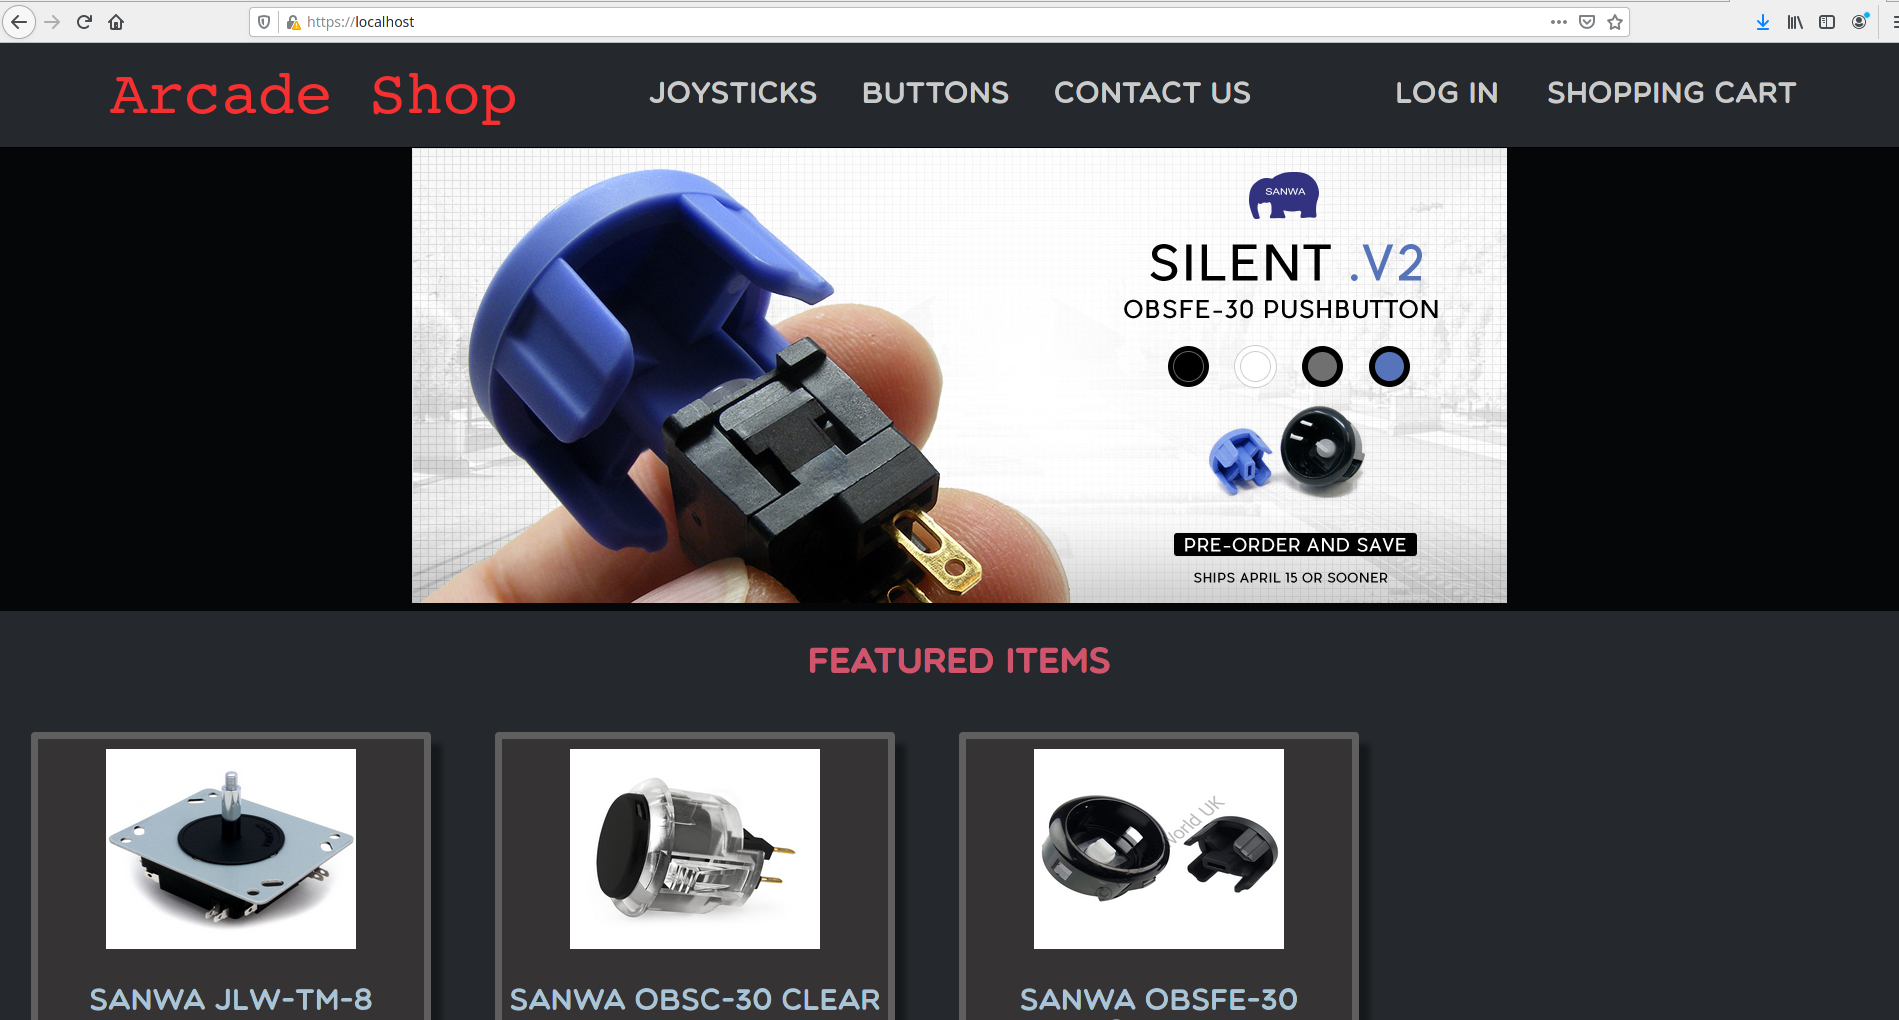
\includegraphics[scale=0.3]{demo_index}
\end{center}
\begin{flushleft}
    A simple view of the menu with different menus available, and a product showcase.
\end{flushleft}

\subsubsection[Registration Success Testing]{Registration Success Testing}
\begin{center}
    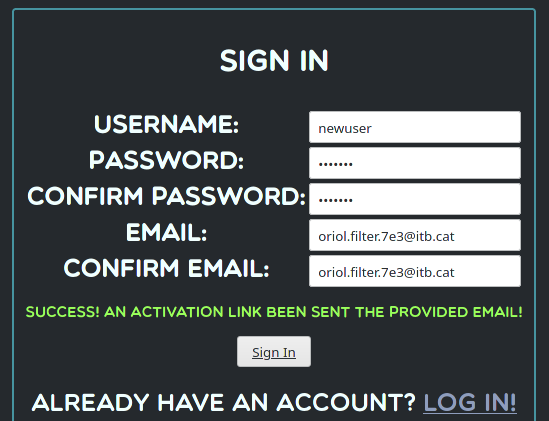
\includegraphics[scale=0.8]{demo_registration_success}
\end{center}
\begin{flushleft}
    We are able to receive responses from the server without the need of updating the page, in this case we were able to succeed in our registration.
\end{flushleft}

\subsubsection[Registration Fail Testing]{Registration Fail Testing}
\begin{center}
    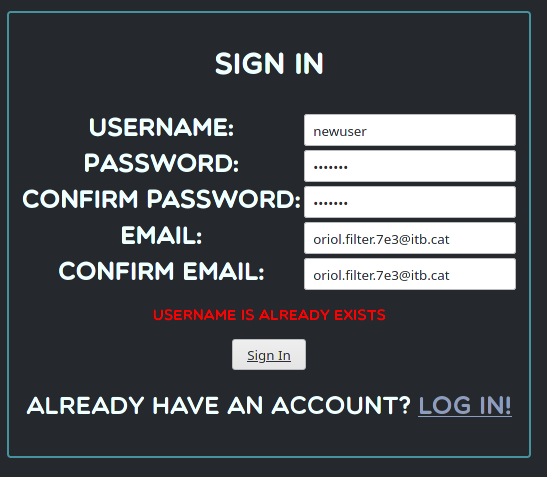
\includegraphics[scale=0.8]{demo_registration_failed}
\end{center}
\begin{flushleft}
    Since our user was already registered we receive a error response.
\end{flushleft}

\subsubsection[Login Unactivated Account Fail Testing]{Login Unactivated Account Fail Testing}
\begin{center}
    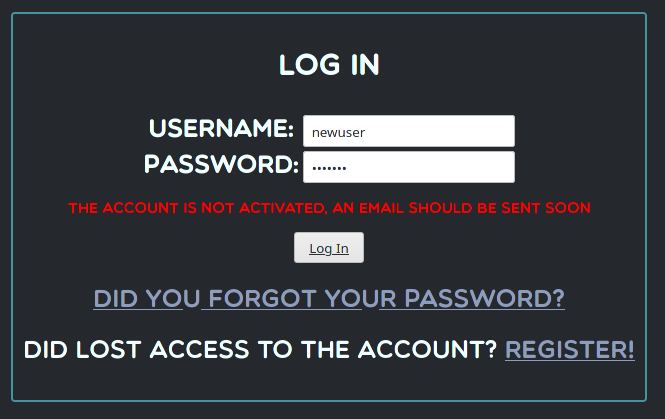
\includegraphics[scale=0.8]{demo_login_failed_unactivated}
\end{center}
\begin{flushleft}
    In order to activate our account, we need to activate our account via the received email.
\end{flushleft}

\subsubsection[Received email Testing]{Received email Testing}
\begin{center}
    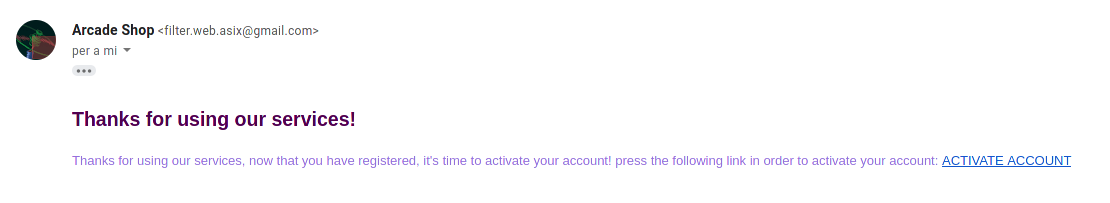
\includegraphics[scale=0.5]{demo_received_email}
\end{center}
\begin{flushleft}
    As expected, we are able to receive a mail to our given email.
\end{flushleft}

\subsubsection[Activate Account Succeed Testing]{Activate Account Succeed Testing}
\begin{center}
    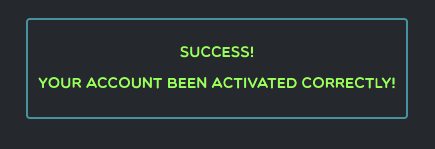
\includegraphics[scale=0.8]{demo_activate_account_succeed}
\end{center}
\begin{flushleft}
    Once we open the link given by the server through the mail, we are able to activate our account.
\end{flushleft}

\subsubsection[Login Success Testing]{Login Success Testing}
\begin{center}
    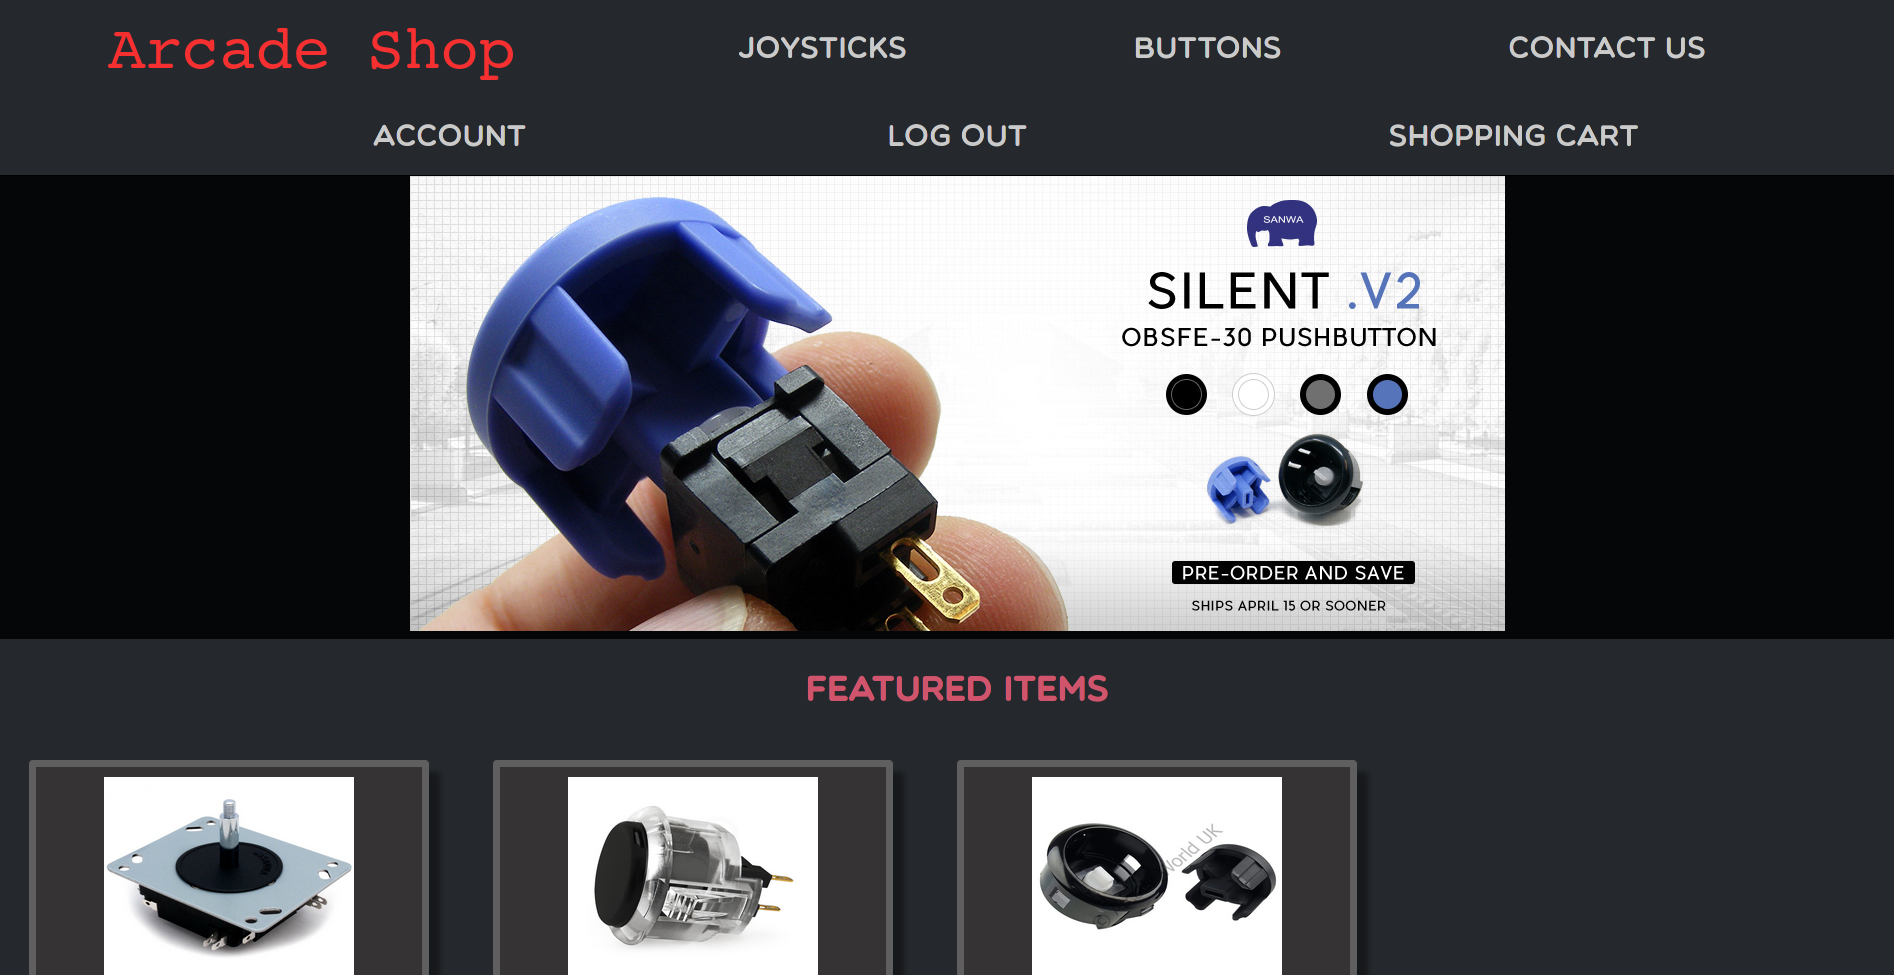
\includegraphics[scale=0.3]{demo_login_succeed}
\end{center}
\begin{flushleft}
    Once we have our account activated, we are able to login correctly, and afterwards we are redirected to the main
    menu, as a proof we can see how the menu it's quite different compared with when we didn't log in.
\end{flushleft}

\subsubsection[Add Shipping Address Fail Testing ]{Add Shipping Address Fail Testing}
\begin{center}
    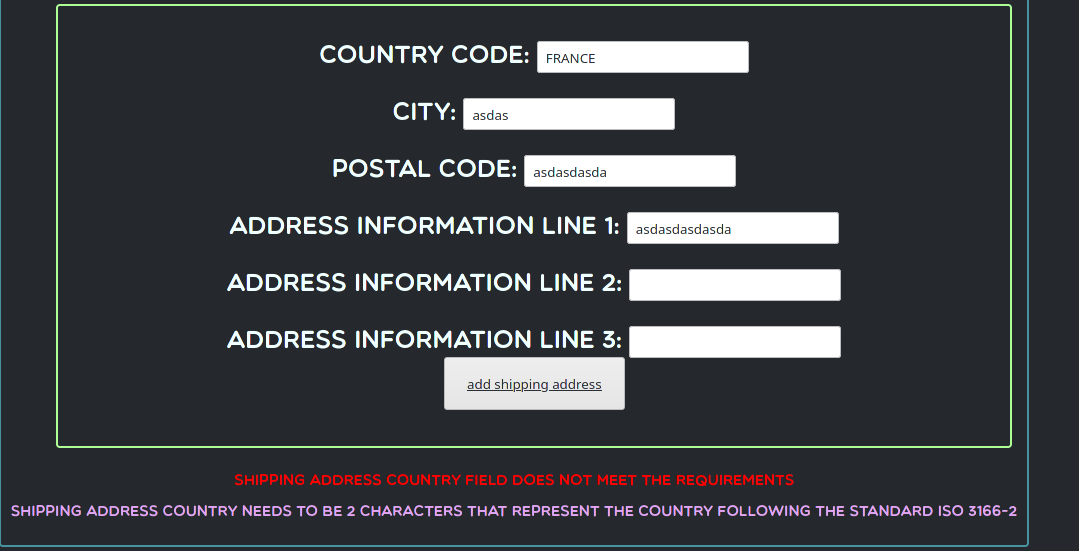
\includegraphics[scale=0.5]{demo_shipping_address_error}
\end{center}
\begin{flushleft}
    Since our country code doesn't consist of 2 characters, it returns error.
\end{flushleft}

\subsubsection[Add Shipping Address Success Testing ]{Add Shipping Address Success Testing}
\begin{center}
    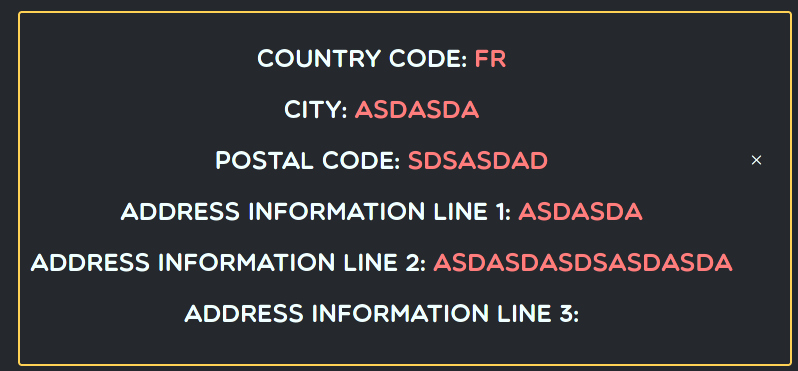
\includegraphics[scale=0.6]{demo_shipping_address_succeed}
\end{center}
\begin{flushleft}
    Once we respect the criteria from the fields, we are able to upload our payment method.
\end{flushleft}

\subsubsection[Remove Shipping Address Success Testing ]{Remove Shipping Address Success Testing}
\begin{center}
    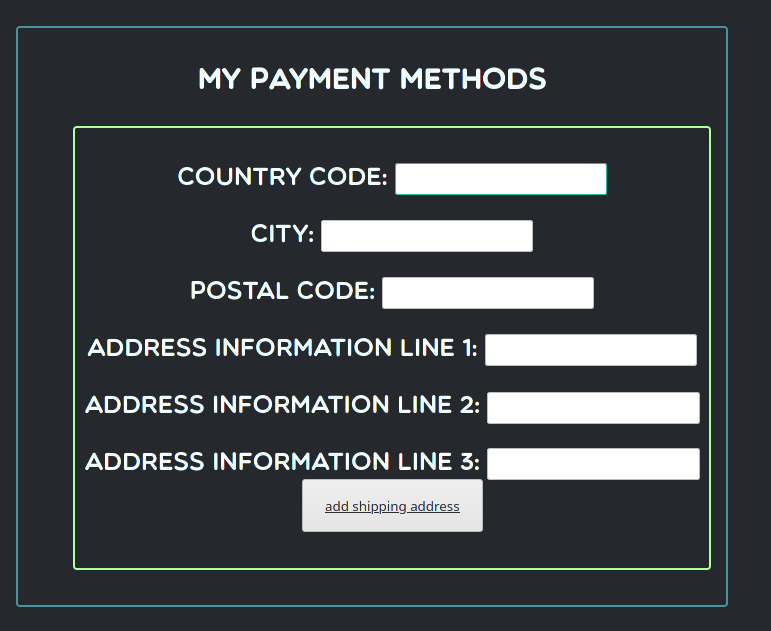
\includegraphics[scale=0.6]{demo_shipping_address_delete_succeed}
\end{center}
\begin{flushleft}
    Deleted the created entries without issues.
\end{flushleft}

\subsubsection[Cookies Testing]{Cookies Testing}
\begin{center}
    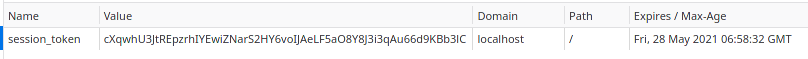
\includegraphics[scale=0.6]{demo_cookies}
\end{center}
\begin{flushleft}
    Checking the cookies, we can see our session token.
\end{flushleft}

